\section{More Dataset Analysis}

\begin{figure}[p]
    \begin{subfigure}
        \centering
        \hspace{-5mm}
        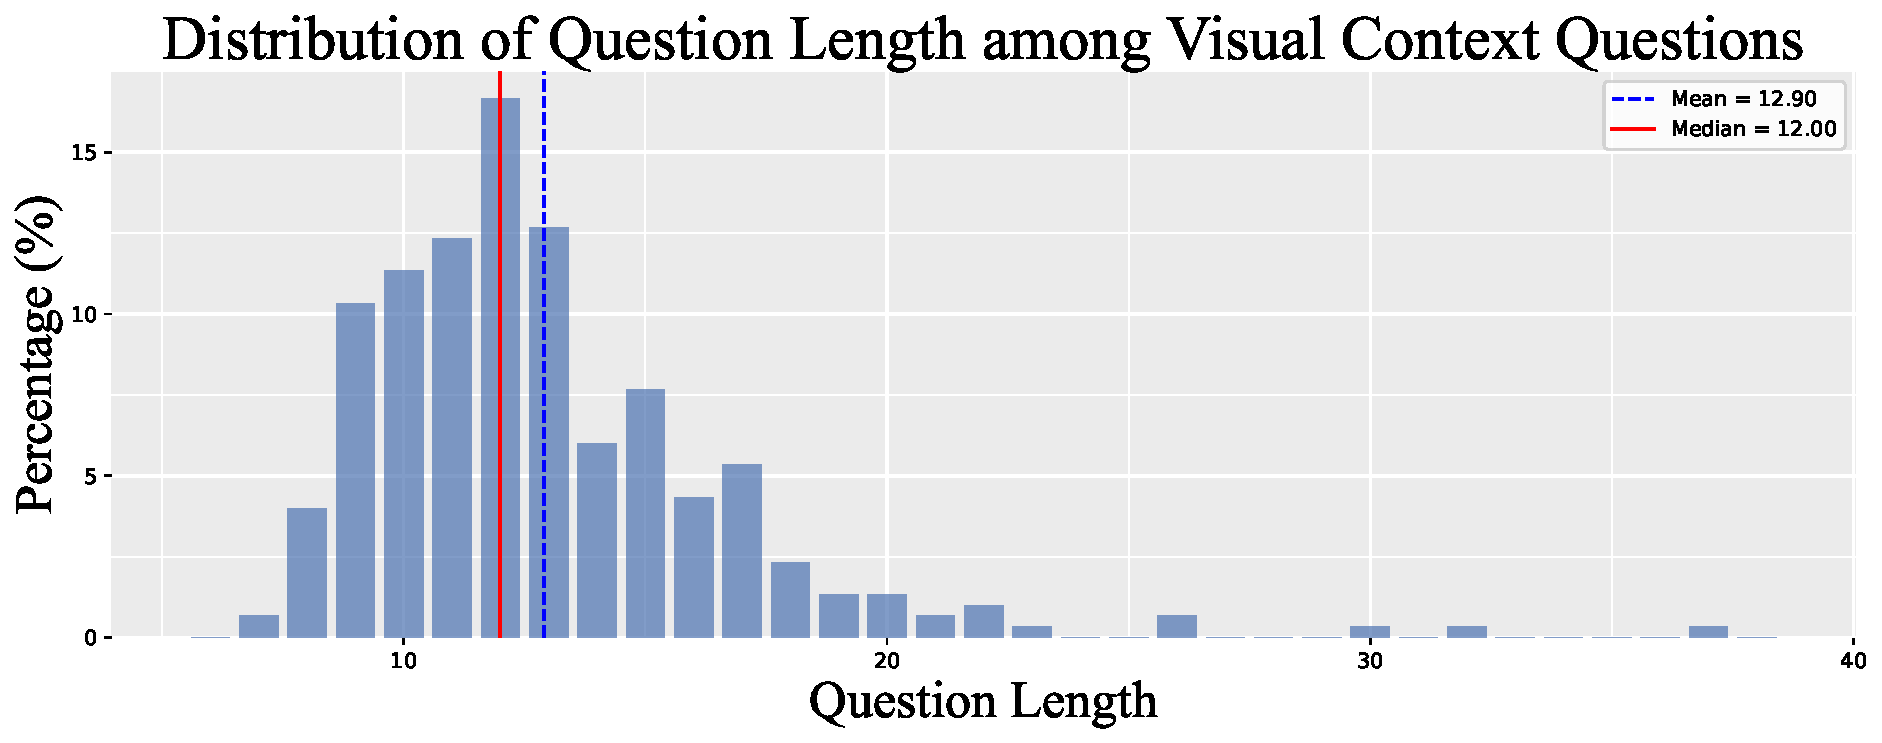
\includegraphics[width=\columnwidth]{appx_figures/locality_questions_distribution.pdf}
        \caption{The distribution of the number of tokens per visual context question in \data  - Part 1 of 3.}
        \label{fig:loc_distribution}
    \end{subfigure}
    \begin{subfigure}
        \centering
        \hspace{-5mm}
        \ContinuedFloat
        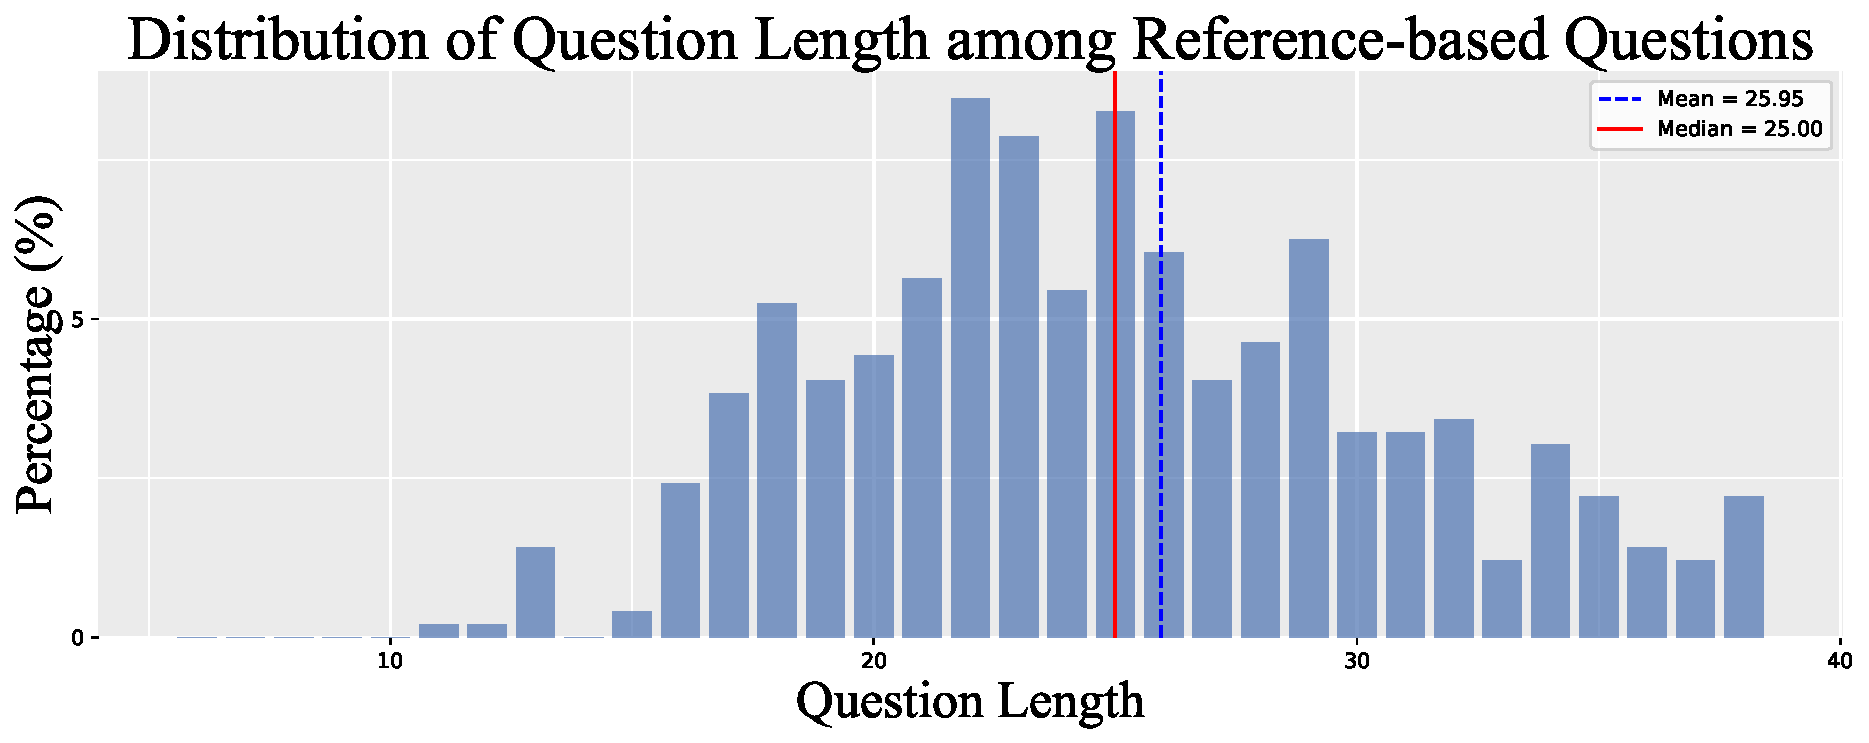
\includegraphics[width=\columnwidth]{appx_figures/detail_questions_distribution.pdf}
        \caption{The distribution of the number of tokens per reference-based question in \data  - Part 2 of 3.}
        \label{fig:detail_distribution}
    \end{subfigure}
    \begin{subfigure}
        \centering
        \hspace{-5mm}
        \ContinuedFloat
        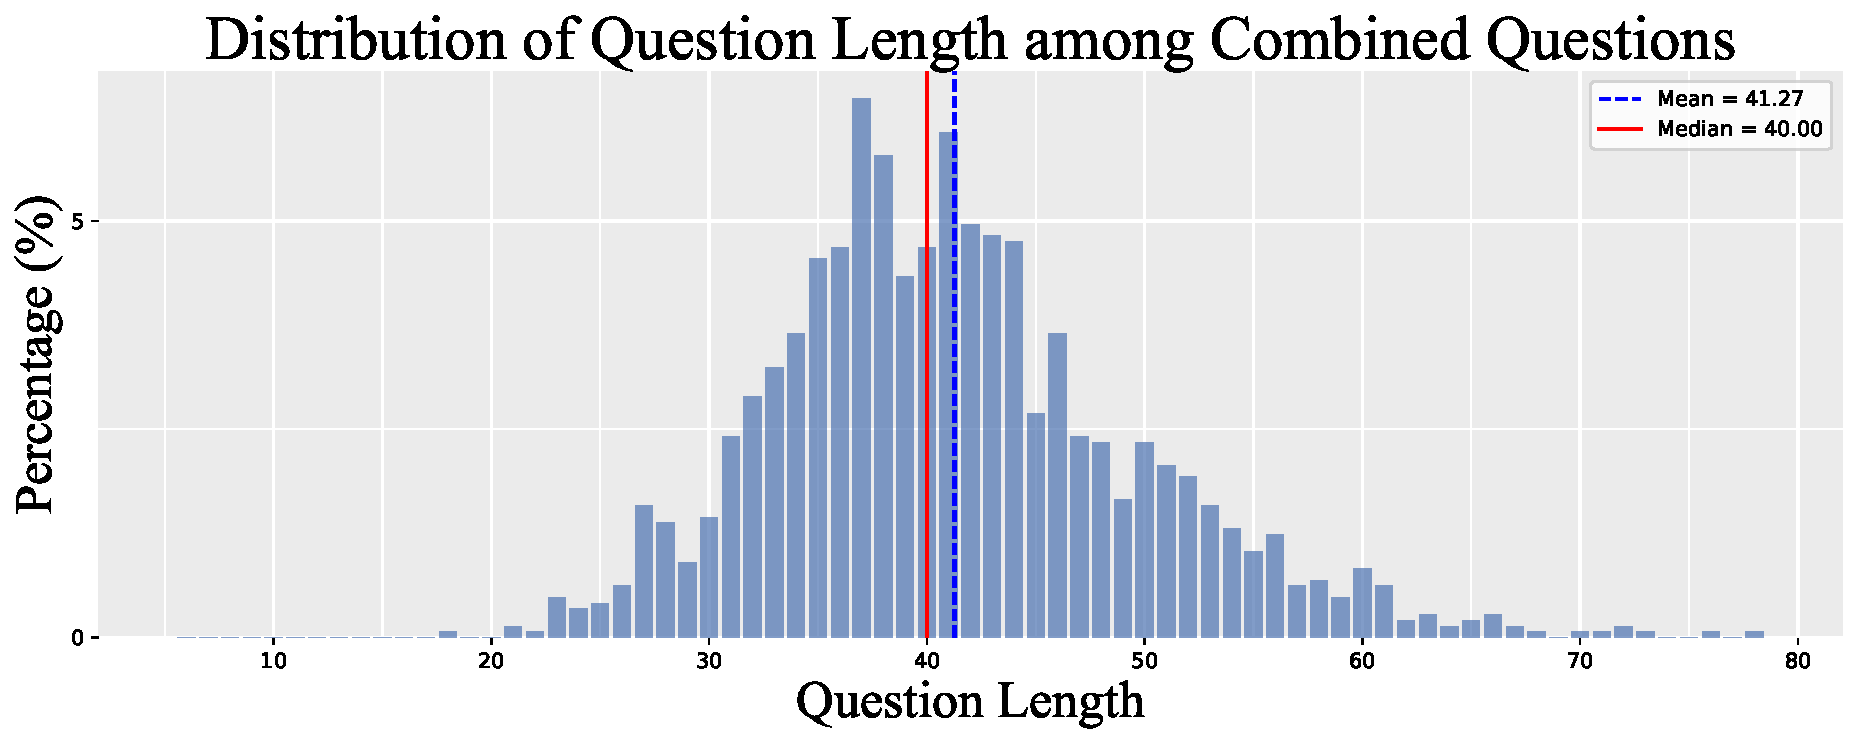
\includegraphics[width=\columnwidth]{appx_figures/combined_questions_distribution.pdf}
        \caption{The distribution of the number of tokens per combined question in \data  - Part 3 of 3.}
        \label{fig:combine_distribution}
    \end{subfigure}


    \label{fig:overall_distribution}
\end{figure}


\paragraph{Question Distribution.} As illustrated in Table \ref{tab:dataset_statistics}, the average question length in \data is 41.27 (in tokens), while the maximum number of tokens in a question is 78 (in tokens).

Figure \ref{fig:combine_distribution} further illustrates the distribution of token counts in all visual context, reference-based, and combined questions, highlighting the diverse distribution of all three types of questions. In these figures, the red solid line represents the median and the blue dashed line represents the mean. From all three distributions, we note that the median and mean are very close in values, implying our dataset is symmetric or only slightly skewed. 


